% !TEX root = ../notes_template.tex

\chapter{조화함수}

마지막 장에서는 다음 내용을 다룬다.

\begin{itemize}
\item[(1)] 라플라스 방정식이라 불리는 편미분방정식의 해가 되는 실함수로서 조화함수를 공부한다.
\item[(2)] 복소해석함수의 실수부와 허수부는 조화함수가 되며
국소적으로 역도 성립한다. 단순연결 영역에서는 전체적으로 역이 성립한다.
\item[(3)] 조화함수와 복소해석함수의 상호관계로부터 도출되는 결과들, 특히
디리클레 방정식이라 불리는 경계값문제에 대한 결과를 살펴본다.
\end{itemize}

\section{조화함수란?}

\begin{salt_definition} \label{def-5-1}
$U$를 $\mathbb R^2$의 열린 부분집합이라고 하자.
함수 $u:U \to \mathbb R$가
$2$차까지의 도함수가 존재하고 연속이면서(줄여서 $u\in C^2$라 한다)
라플라스 방정식
\[
(\Delta u)(x,y) := \dfrac{\partial^2 u}{\partial x^2} (x,y) 
+ \dfrac{\partial^2 u}{\partial y^2} (x,y) = 0,
\quad
(x,y) \in U
\]
을 만족하면, {\bf 조화함수}(harmonic function)라고 한다.
\end{salt_definition}

\begin{salt_example}\label{example-5-1}
$U=\mathbb R^2$라 하자.
함수 $u: U\to \mathbb R$가 모든 $(x,y)\in \mathbb R^2$에서
$u(x,y) = x^2-y^2$로 주어지면,
\begin{align*}
 &\dfrac{\partial u}{\partial x} = 2x, \hphantom{-} \quad  \dfrac{\partial^2 u}{\partial x^2} = 2, \\
 &\dfrac{\partial u}{\partial y} = -2y, \quad   \dfrac{\partial^2 u}{\partial y^2} = -2
\end{align*}
이므로 $\dfrac{\partial^2 u}{\partial x^2} (x,y) 
+ \dfrac{\partial^2 u}{\partial y^2} (x,y) = 2-2=0$이다.
$\mathbb R^2$에서 $u\in C^2$이고 $\Delta u=0$이므로 $u$는 조화함수이다.
\hfill $\diamondsuit$
\end{salt_example}

물론 모든 함수가 조화함수는 아니다.

\begin{salt_example}\label{example-5-2}
$(x,y)\in \mathbb R^2$에서 $\tilde u(x,y) = x^2+y^2$으로 정의된 함수  $\tilde u$를 생각하면,
\[
\dfrac{\partial^2 \tilde u}{\partial x^2} (x,y) 
+ \dfrac{\partial^2 \tilde u}{\partial y^2} (x,y) = 2+2=4\ne 0.
\]
따라서 $\Delta \tilde u$는 $\mathbb R^2$의 모든 점에서 $0$이 되지 않기에
$\tilde u$는 $\mathbb R^2$의 어떤 열린 부분집합에서도 조화함수가 될 수 없다.
\hfill $\diamondsuit$
\end{salt_example}

\begin{salt_exercise}\label{ex-5-1}
다음 함수 $u$가 주어진 열린집합 $U$에서 조화함수임을 보여라.
\begin{itemize}
\item[(1)] $u(x,y) = \log (x^2+y^2)$, $U = \mathbb R^2\setminus \{(0,0)\}$
\item[(2)] $u(x,y) = e^x\sin y$, $U=\mathbb R^2$.
\end{itemize}
\end{salt_exercise}

\begin{salt_exercise}\label{ex-5-2}
열린집합 $U$에 정의된 모든 조화함수의 집합 $\Har(U)$는
점별 연산에 대하여 실벡터공간을 이룸을 보여라.
\end{salt_exercise}

\begin{salt_exercise}\label{ex-5-3}식
조화함수의 점별 곱으로 만든 함수도 조화함수가 되는가?
\end{salt_exercise}

{\bf 왜 조화함수에 신경써야 하는가?}

조화함수는 라플라스 방정식을 만족하기 때문에 중요한데,
라플라스 방정식은 여러가지 이유 중 다음 두 가지 때문에 특히 중요하다.
\begin{itemize}
\item[(1)] 라플라스 방정식은 편미분방정식(PDE)의 3가지 유형 중에서 
타원형 방정식이라는 중요한 유형에 속한다.
\begin{center}
\begin{tabular}{ |c|c| } 
 \hline
PDE 유형 & 예 \\ \hline \hline
타원형 & 라플라스 방정식 
$\dfrac{\partial^2 u}{\partial x^2} 
+ \dfrac{\partial^2 u}{\partial y^2} =0$ \\[1ex] \hline
포물형 & 확산 방정식 $\dfrac{\partial u}{\partial t} 
+ \dfrac{\partial^2 u}{\partial x^2} =0$ \\[1ex] \hline
쌍곡형 & 파동 방정식 $\dfrac{\partial^2 u}{\partial t^2} 
- \dfrac{\partial^2 u}{\partial x^2} =0$ \\[0.5ex]
\hline
\end{tabular}
\end{center}
\item[(2)] 라플라스 방정식은 많은 응용분야에서 사용된다.
다음과 같이 물리학에서 사용되는 예를 살펴보자.
유체역학에서 유체흐름의 ``속도 포텐셜(velocity potential)''은
라플라스 방정식을 만족한다. 한편, 정전기학에서는
정전기 전위(electronic potential)가 라플라스 방정식을 만족한다.
라플라스 방정식은 확률과정(stochastic process)과도 중요한 연결고리를 갖는다.
아래에서 이를 간단히 알아보자.
열린 단위원판 $\mathbb D:= \{z\in \mathbb C\,:\, |z|<1\}$을 생각하자.
입자가 한점 $z\in\mathbb D$에서 브라운 운동을 따른다고 하자.
(예를 들면, 무작위 운동을 만드는 물분자에 의해 충격받는 물 속의
꽃가루를 생각하자.)
직관적으로 무작위 운동으로 언젠가는 입자가 $\mathbb D$의 경계 
$\mathbb T:= \{ z\in \mathbb C \,:\, |z|=1 \}$를 벗어난다.
$z$에서 출발한 입자가 처음으로 단위원 $\mathbb T$를 벗어나는 
점을 $\zeta_z$라고 하자. 그러면 확률변수 $\zeta_z$는 단위원 위에 표시된다.
그림 \ref{fig-5-1}을 참고하라.
\begin{figure}[h!]
\begin{center}
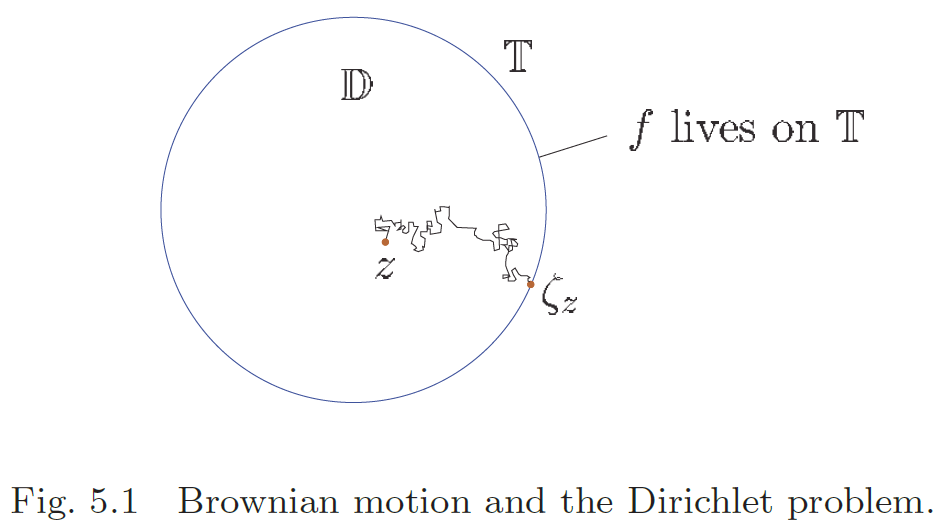
\includegraphics[width=0.6\textwidth]{./SaltChapter/fig-5-1}
\end{center}
\caption{브라운 운동과 디리클레 문제}
\label{fig-5-1}
\end{figure}
이제 연속함수 $f:\mathbb T \to \mathbb R$이 주어졌다고 하자.
그러면 $f(\zeta_z)$를 $\mathbb T$에 정의된 실수 값을 갖는 확률변수로 생각할 수 있다.
그 기댓값을 $\mathbb E(f(\zeta_z))$으로 표기하자.
이 값은 어디에서 출발하는지에 따라 달라진다. 즉, $z$에 의존하는 값이다.
$u:\mathbb D \to \mathbb R$을 $u(z) =\mathbb E(f(\zeta_z))$ ($z\in \mathbb D$)로 
정의하자. 이 때, $u$는 조화함수이고 실제로 디리클레 문제의 해가 됨이 알려져 있다.
이는 경계값 문제로 경계 $\mathbb T$에서 함수 $f:\mathbb T \to \mathbb R$가 
주어져 있을 때, $\mathbb T$의 내부 $\mathbb D$에서는 라플라스 방정식을 만족하고
경계 $\mathbb T$까지 연속함수로 확장되어 $f$와 일치하는 함수 $u$를 찾는 문제이다.
\[
\begin{cases}
\Delta u = 0, & \mathbb D\text{\,에서},\\
u\big|_{\mathbb T}= f.
\end{cases}
\]
\end{itemize}

\section{조화함수와 복소해석함수의 연결고리는 무엇인가?}

조화함수는 단지 실해석의 영역에 속해야 하는 것처럼 보일 수 있다.
이 절에서는 복소해석학에 대한 연구를 충분히 정당화할 수 있는 두가지 결과를 알아볼 것이다.
개략적으로 말하면, 열린집합에 정의된 조화함수는 국소적으로 복소해석함수의 실수부라는 
조건과 동치이다.





